\section{Технологический раздел}


\par В данном разделе будет произведен выбор и обоснование языка программирования, среди разработки, а также задействованных библиотек. Помимо этого также будут описаны задействованные данные и разработана структура программного обеспечения.


\subsection{Выбор и обоснование языка программирования, среды
разработки и задействованных библиотек}

\par На следующем этапе исследования были реализованы прогнозные модели. Для этого
использовался язык программирования Python. Интегрированной средой разработки был выбран Google Colaboratory – облачный сервис для проведения исследований в машинном и
глубоком обучении, который представляет собой онлайн–блокнот Jupyter, не требующий дополнительных установок и позволяющий запускать код на графическом процессоре Nvidia
Tesla V100, что значительно ускоряет процесс обучения моделей.
В исследовании использовались следующие библиотеки:

\begin{itemize}[leftmargin=1.6\parindent]
    \item[---] \textit{Scikit-learn}. Данная библиотека содержит готовые реализации многих алгоритмов машинного обучения, а также метрики оценивания алгоритмов;
	\item[---] \textit{Matplotlib}. Использовалась для построения графиков;
	\item[---] \textit{Keras}. Нейросетевая библиотека, предназначенная для оперативной имплементации сетей глубокого обучения. Она содержит готовые слои и умеет объединять их между собой в сеть, обучать и реализовывать с ее помощью прогнозы;
	\item[---] \textit{TensorFlow}. Библиотека машинного и глубокого обучения позволяет оптимизировать вычисления, производимые во время обучения;
	\item[---] \textit{Pandas}. Библиотека предназначенная для обработки и анализа данных;
	\item[---] \textit{XGBoost}. Библиотека предназначенная для повышения градиента;
	\item[---] \textit{Numpy}. Библиотека для поддержки больших многомерных массивов данных.
\end{itemize}

\subsection{Задействованные данные}

\par В основе данной работы лежит эмпирическое исследование курса акций Bank of China на фондовом рынке. Данные о цене акций находятся в открытом доступе и отобраны в диапозоне с первого января 2007 года по 31 марта 2022 года. Один день торгов является по своей сущносте единицей последовательности временного ряда. Сформированный на их основе трениворочный и тестовый набор отображены на рисунке под номером \ref{fig:close-price}. Процентное соотношение тренировочного и тестового набора составляет 95\% и 5\% соответственно.

\begin{figure}[hbtp]
  \centering
  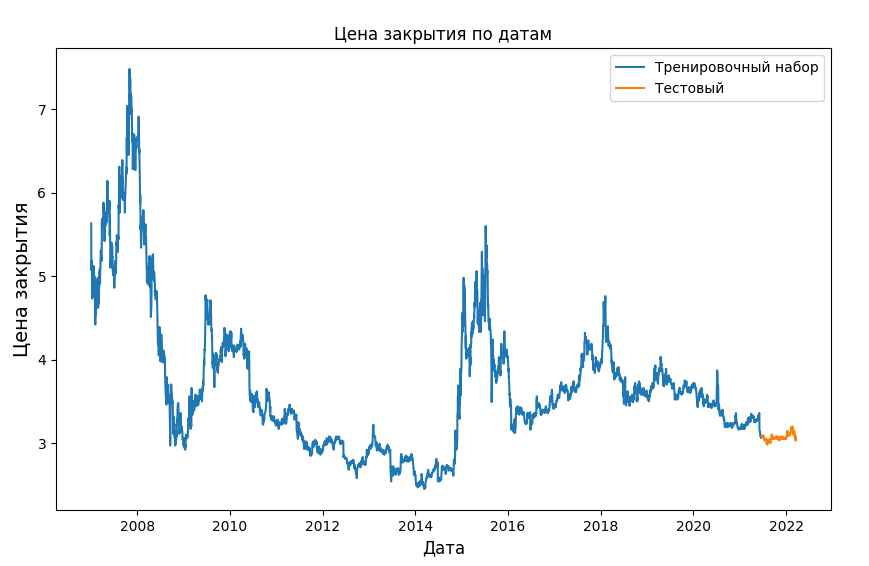
\includegraphics[width=\textwidth]{img/Close_price.png}
  \caption{Курс акций Bank of China, разбитый на тренировочный и тестовый набор.}
  \label{fig:close-price}
\end{figure}

\newpage

\par Важно отметить, что данные о цене акций состоят из таких параметров, как цена открытия и закрытия, наибольшая и наименьшая цена за день и так далее. Затем эти данные проходят через модель ARIMA. Полученная в результате последовательность совместно с изначальными данными является характеристиками временного ряда, отображенная схематично на рисунке \ref{fig:feature}. 

\begin{figure}[hbtp]
  \centering
  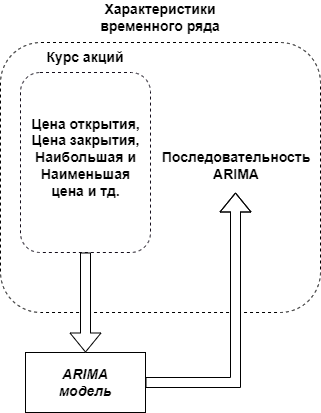
\includegraphics[width=0.3\textwidth]{img/features.png}
  \caption{Схема составных частей характеристик временного ряда.}
  \label{fig:feature}
\end{figure}

\par Входными данными нейросетевого модуля является двумерная матрица размером количества характеристик временного ряда на временное окно. Шириной временного окна в данном случае является число 20.

\newpage

\subsection{Структура разработанного программного комплекса}

\par Структура разработанного программного комплекса представлена на рисунке \ref{fig:final-scheme}. Тренировка проходила в течение 50 эпох для обеспечения стабильного результата точности и потерь. В качестве функции оптимизации для модели была использована функция Adam (адаптивная оценка момента). Количество слоев LSTM 5 с размером в 64. Модель тренируется при помощи выбывания (dropout), уровень которого составляет 0.3.

\begin{figure}[hbtp]
  \centering
  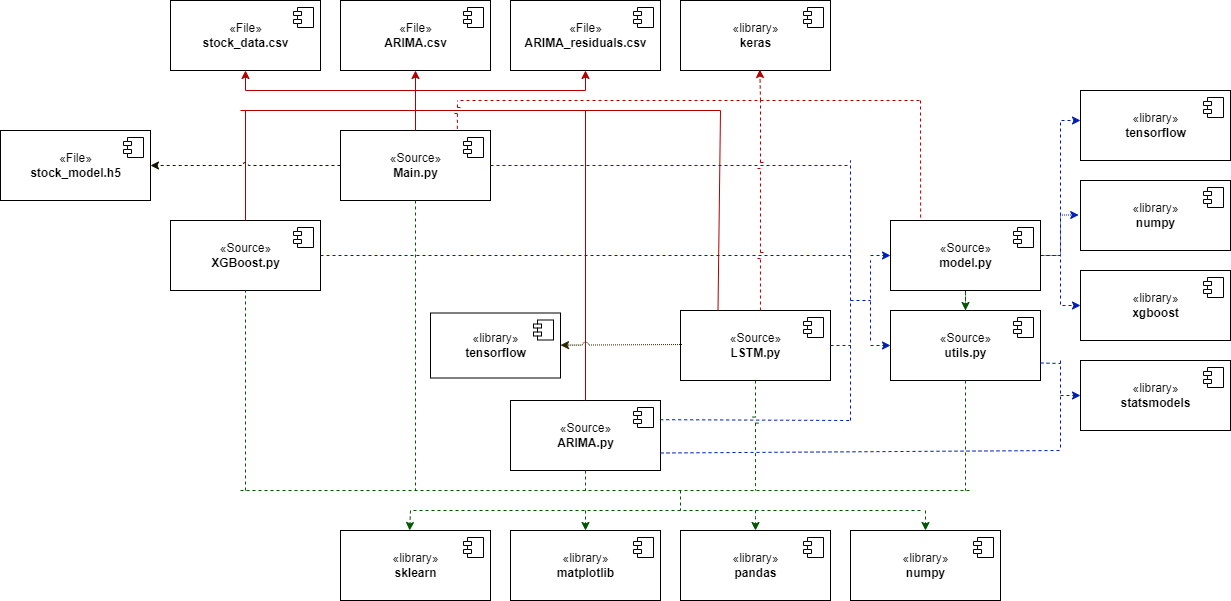
\includegraphics[width=\textwidth]{img/software-structure .png}
  \caption{Структура разработанного программного комплекса.}
  \label{fig:final-scheme}
\end{figure}
\newpage
\subsection{Выводы из технологического раздела}
\par В данном разделе был произведен выбор и обоснование языка программирования, среди разработки, а также задействованных библиотек. Помимо этого также были подробно описаны задействованные данные и разработана структура программного обеспечения.
\pagebreak